% besdoc.tex V1.0, 17 March 2011

\documentclass[times,mee,doublespace,]{besauth2}
%%\documentclass[times,mee,]{besauth}

\newcommand{\journalnamelc}{British Ecological Society}
\newcommand{\journalabb}{British Ecological Society}
\newcommand{\journalclassshort}{BES}
%%\newcommand{\journalname}{British Ecological Society}
\usepackage{epstopdf}

\usepackage{moreverb}

\usepackage[colorlinks,bookmarksopen,bookmarksnumbered,citecolor=red,urlcolor=red]{hyperref}


\usepackage{lineno}

\newcommand\BibTeX{{\rmfamily B\kern-.05em \textsc{i\kern-.025em b}\kern-.08em
T\kern-.1667em\lower.7ex\hbox{E}\kern-.125emX}}

\bibpunct[; ]{(}{)}{;}{}{}{,}

\def\volumeyear{2014}
\def\VOC{VO}

\begin{document}
\runningheads{P.~B.~Conn et al.}{Space-time abundance models}

\papertype{Article}

\title{Using spatio-temporal statistical models to estimate animal abundance and infer ecological dynamics from count data} %\footnotemark[2]}

\author{P.~B. ~Conn\affil{1}\corrauth, D.~S. ~Johnson\affil{1}, J.~M. ~Ver Hoef\affil{1}, M.~B. ~Hooten\affil{2}\affil{3}\affil{4},  J. ~M. ~London\affil{1}, P. ~L. ~Boveng\affil{1}}


\address{\affilnum{1}National Marine Mammal Laboratory, Alaska Fisheries Science Center, NOAA National Marine Fisheries Service, 7600 Sand Point Way NE, Seattle, WA 98115 USA;\affilnum{2}U.S. Geological Survey, Colorado Cooperative Fish and Wildlife Research Unit, Colorado State University, Fort Collins, CO 80523 USA;\affilnum{3} Department of Fish, Wildlife, and Conservation Biology, Colorado State University, Fort Collins, CO 80523 USA;\affilnum{4}Department of Statistics, Colorado State University, Fort Collins, CO 80523 USA}

\corraddr{paul.conn@noaa.gov}

\begin{abstract}
 %\noindent {\emph{Summary}}
\small
\begin{enumerate}
\item  Ecologists often estimate animal abundance using models fit to survey counts. Such models often require that animal density remains constant across the landscape where sampling is being conducted.  This assumption is problematic for animals inhabiting dynamic landscapes or otherwise exhibiting considerable spatio-temporal variation in density, and may be an impediment to inference about how changes in environmental conditions affect animals' spatial distribution.  A variety of models have been developed for analyzing spatio-temporal variation in count data, but there has been little comparison of the efficacy of alternative modeling approaches when the goal is to estimate animal abundance or examine species-habitat relationships.

\item We review several concepts from the burgeoning literature on spatio-temporal statistical models, including the nature of the temporal structure (i.e., descriptive or dynamical) and strategies for dimension reduction to promote computational tractability.  We also review several features as they specifically relate to abundance estimation, including boundary conditions, population closure, choice of link function, and extrapolation of predicted relationships to unsampled areas.

\item We compare a suite of novel and existing spatio-temporal hierarchical models for animal count data that permit animal density to vary over space and time.  Models varied by the nature of the temporal structure (i.e., descriptive or dynamical), and whether total expected abundance was assumed constant over time (a pseudo-closure assumption).  We gauge the relative performance (bias, precision, computational demands) of alternative spatio-temporal models when confronted with simulated and real datasets from dynamic animal populations.  For the latter, we analyze spotted seal counts from an aerial survey of the Bering Sea where the quantity and quality of suitable habitat (sea ice) changed dramatically while surveys were being conducted.

\item Later...

\end{enumerate}


% Word count: 5332
\end{abstract}

\keywords{Animal abundance, resource selection, process convolution, spatio-temporal model, transect survey}

\maketitle \linenumbers

\def\VAR{{\rm Var}\,}
\def\COV{{\rm Cov}\,}
\def\Prob{{\rm P}\,}



\section{Introduction}

A tacit assumption in many models for animal transect data is that animal density remains constant over
the landscape while sampling is being conducted.  This assumption is clearly unrealistic for populations that inhabit dynamic landscapes or whose spatial distribution varies considerably over the course of a study. For instance, the distribution and abundance of bird species inhabiting agricultural landscapes can vary substantially within seasons due to cultivation and harvesting practices \citep{MillerEtAl11jwm}, as can abundance of bird and amphibian populations that are dependent on dynamic wetland environments \citep{MurkinEtAl1997,BabbittTanner2000}.   Our own interest in spatio-temporal variation in animal abundance stems from involvement in surveys of ice-associated seals, where the quantity and distribution of suitable habitat (seasonal sea ice) changes dramatically on the scale of weeks or even days \citep{VerHoefJansen2007,VerHoefEtAl2014}.

Early development of models for analysis of animal transect data \citep[see e.g.][and references therein]{BucklandEtAl2001} focused on design-based estimation \citep[cf.][]{Cochran1977}, which is perhaps the most simple and reliable approach for obtaining ``snapshot" estimates of abundance, provided that the spatial configuration of animal density does not vary appreciably while the study is being conducted and that a sampling frame (e.g. systematic, stratified random samples) can be developed and strictly adhered to.  More recently, model-based approaches for analyzing animal abundance from transect counts \citep[e.g.][]{HedleyBuckland2004,VerHoefJansen2007,JohnsonEtAl2010} have become more prevalent. Although these approaches require additional (often distributional) assumptions, model-based inference permits greater flexibility because sampling effort can be allocated at different times and locations than originally planned, and because features such as temporal \citep{Moore2011} and spatial \citep[see e.g.][]{MillerEtAl2013} autocorrelation can be included and visualized.

Development of model-based estimation procedures for transect data have largely focused on inclusion of spatial variation in abundance without as much consideration of temporal variation.  Notable exceptions include \citet{VerHoefJansen2007}, who included changing habitat covariates and additive spatial and temporal effects in count models for harbor seals; \citet{MillerEtAl11jwm}, who allowed bird density to rely on habitat covariates that varied between sample occasions \citep[using an N-mixture formulation; see][]{Royle2004}; \citet{Moore2011}, who allowed the modelled density of fin whales to vary among years and spatial strata; and \citet{VerHoefEtAl2014}, who conceptualized phocid seal counts as a function of both changing habitat covariates and spatially autocorrelated random effects.  Hierarchical generalized linear mixed models incorporating both spatial and temporal effects are also prevalent in analysis of population trend from count data \citep[e.g.][]{SauerLink2011,RossEtAl2012}, but it is not often possible to scale up from these models to the estimates of absolute density or abundance that are often needed for population management.

The statistical literature on spatio-temporal models has exploded in recent years (see \citeauthor{CressieWikle2011} \citeyear{CressieWikle2011} for a review), and in theory it would be possible to embed a large number of spatio-temporal models for animal density into model-based estimation procedures for transect counts.  \citet{CressieWikle2011} categorize such models as either descriptive, where spatio-temporal autocorrelation is codified by allowing positive covariance at times and locations that are close together, or dynamical (i.e. process-based), where the investigator uses knowledge of the study system to help specify a dynamical model governing the evolution of the spatio-temporal process over time \citep[e.g. via difference equations;][]{WikleHooten2010}.  Spatio-temporal models often include one or more strategies for dimension reduction to ease computational burden \citep[of which there are many; for a review see][]{Wikle2010}.  As such, it will not be possible to enumerate all possible approaches for incorporating spatio-temporal structure into abundance models.
Instead, we start by reviewing recent work in this field, aiming to provide ecologists with intuition on the flavors of spatio-temporal models currently available in the literature, providing connections with relevant ecological theory where applicable \citep[e.g. with ideal free distributions;][]{FretwellLucas1970}.

Next, we turn our focus to spatio-temporal modelling considerations as they relate specifically to abundance estimation.  These include boundary conditions (emigration/immigration from the study area), demographic closure (population increases/decreases due to mortality or reproduction), choice of link function, and extrapolation of fitted relationships to unsampled areas. After delineating a (by no means exhaustive) suite of spatio-temporal models for abundance estimation (including novel formulations embodying resource selection and permitting a form of population closure), we illustrate the consequences of different modelling choices by analyzing both simulated data and seal count data from transects over the Bering Sea. In both cases, the quantity and quality of available habitat changes dramatically while surveys are being conducted.

\section{Spatio-temporal models for count data}

Animal count data are most often obtained on areal sample units (i.e., in discretized space) and at discrete points in time.  Even if sampling is not instantaneous, a common convention in spatio-temporal models is to discretize time at some level (e.g., daily) and to treat all counts gathered in a given day as if they occurred instantaneously. In the following, we shall follow these conventions, and shall model both the abundance of animals and observed transect counts by appealing to specific points in time $t \in  \{ 1,2,\hdots,T \} $ and specific sample units $s \in \{ 1,2,\hdots,S \}$.  For simplicity, we shall assume that all sampling units are the same size (this requires apportioning counts into respective sampling units whenver transects cover more than one sample unit in the same survey).  Our task shall be to construct plausible spatio-temporal models that describe how a sample of observed counts at a subset of $n$ locations and times $\{ <s_1,t_1>,<s_2,t_2>,\hdots <s_n,t_n> \}$ are related to absolute abundance $N_{s,t}$ at all times and sample units.

All spatio-temporal models that we examine relate observed counts, $C_k$, obtained at a limited number of times and sample units, to a hidden spatio-temporal process $\mu_{s,t}$ that is defined over all sample units and times through a standard probability mass function $f$, link function $g$, covariates ${\bf x}$, and parameters $\boldsymbol{\theta}$ (throughout this article we shall use bold symbols to denote vectors and matrices).  For example, the formulation
\begin{eqnarray}
  {\bf C} & \sim & \textrm{Poisson}({\bf \lambda}), \nonumber \\
  \boldsymbol{\lambda} & = & \exp \left( {\bf o} + {\bf H}\boldsymbol{\mu} \right) \label{eq:basic-mod}
\end{eqnarray}
specifies that counts are Poisson distributed with a log link function on abundance intensity. Following \citet{WikleHooten2010}, we use the matrix ${\bf H}$ to map from the full set of $ST$ values of $\mu_{s,t}$ to the smaller set of $n$ counts. We also include log offsets ${\bf o}$ to allow for differences in the amount of area surveyed (this could also be used to help model detection probability when detectability is less than 1.0; see Discussion).  In practice, more flexible distributional forms could be considered, such as the negative binomial or Conway-Maxwell Poisson \citep{WuEtAl2013}, but our focus here is in describing general forms for the spatio-temporal process $\mu_{s,t}$ and we shall use the Poisson as a convenient form for $f$ throughout the remainder of this article.

Models with the form of eqn \ref{eq:basic-mod} can sometimes be analyzed directly via maximum likelihood, but introducing even moderate complexity in models for $\mu_k$ can make computation intractable.  To preserve flexibility, we prefer to specify prior distributions for model parameters and to conduct Bayesian inference \citep[see e.g.][]{GelmanEtAl2004} on complete data likelihoods \citep{Dempster1977}.   We follow the tradition of \citet{Berliner1996} in expressing the posterior distribution associated with eqn \ref{eq:basic-mod} as consisting of an observation model, a process model, and a set of
prior distributions.  Letting $[a|b]$ denote the conditional distribution of $a$ given $b$, we write the joint posterior distribution for parameters $\boldsymbol{\theta}$ and latent variables $\boldsymbol{\mu}$ (up to proportionality constant) as
\begin{eqnarray}
  [\boldsymbol{\mu},\boldsymbol{\theta} | {\bf x},{\bf C},{\bf o}] & \propto & [{\bf C} | {\bf o}, \boldsymbol{\mu}] [\boldsymbol{\mu} | \boldsymbol{\theta},{\bf x}] [\theta].
  \label{eq:hmod}
\end{eqnarray}
Here, $[{\bf C} | {\bf o}, \boldsymbol{\mu}]$ simply describes the Poisson observation model (the first line in eqn. \ref{eq:basic-mod}), $[\boldsymbol{\mu} | \boldsymbol{\theta},{\bf x}]$ describes the process model (how latent abundance varies over space and time), and $[\theta]$ describes prior parameters.  Although care must be taken in formulating observation and prior parameter models, we now turn to describing different ways of formulating the spatio-temporal process model before discussing ways of using dimension reduction to decrease computational burden.

\subsection{Descriptive vs. dynamical formulations}

\citet{CressieWikle2011} classify spatio-temporal models into two types: descriptive and dynamical.  The development of descriptive spatio-temporal models largely follows the development of spatial and time series models, where there is an a priori expectation that system states (in our case, $\mu_{s,t}$) close together in space or time should be similar to one another.  In descriptive models, this expectation is often codified by specifying a covariance function that decreases as a function of distance (where distance can be either in space or time).  For instance, the model
\begin{eqnarray}
  \mu_{s,t} = {\bf X}_{s,t} \boldsymbol{\beta} + \eta_s + \gamma_t + \kappa_{s,t} + \epsilon_{s,t} \label{eq:glmm}
\end{eqnarray}
might be used to indicate that the expected number of animals at location $s$ at time $t$ is a function of covariates ${\bf X}_{s,t}$ and regression parameters $\boldsymbol{\beta}$, a purely spatial random effect ($\eta_s$), a purely temporal random effect ($\gamma_t$), a spatio-temporal random effect ($\kappa_{s,t}$), and Gaussian white noise $\epsilon_{s,t}$.  Statisticians have developed a large number of models to impart purely spatial \citep[e.g. geostatistical models, Gaussian Markov random fields (GMRFs); see e.g.][]{Cressie1993,BanerjeeEtAl2004,RueHeld2005} or temporal \citep[e.g. AR(p) processes and ARIMA models;][]{BoxEtAl2008,PradoWest2010} autocorrelation to random effects.
Similar approaches can be used to define spatio-temporal covariance functions \citep{CressieWikle2011} for the $\kappa_{s,t}$ random effects.

By contrast, dynamical spatio-temporal models attempt to model the mechanism by which the spatio-temporal process evolves over time.  In spatio-temporal models for physical processes (e.g. atmospheric processes), the evolution of the spatio-temporal process is largely governed by the laws of physics, which can be represented with ordinary or partial differential equations \citep{WikleEtAl2001,WikleHooten2010}.  Discrete time approximations to such equations can provide much more meaningful structure than simple descriptive models, although descriptive model features can still be used to account for residual spatio-temporal autocorrelation.  In ecology, dynamical spatio-temporal models have been used to model invasive species spread \citep{Wikle2003,HootenEtAl2007,HootenWikle2008}.  Even though invasive species do not necessarily subscribe to a single succinct ``law" that governs their spread, physical models for advection-diffusion processes are still incredibly useful for describing and constraining evolution of the spatio-temporal process.

Coming back to the problem of estimating animal abundance, consider a dynamical model for $\mu_{s,t}$ that takes on the form
\begin{eqnarray}
  [\boldsymbol{\mu}|\boldsymbol{\theta}] & = & [\boldsymbol{\mu}_1 | \boldsymbol{\theta}] \prod_{t=2}^T [\boldsymbol{\mu}_t | \boldsymbol{\mu}_{t-1},\boldsymbol{\theta}].
  \label{eq:mu}
\end{eqnarray}
where subscripts in this case denote time (so that $\boldsymbol{\mu}_t$ describes a collection of $\mu_{s,t}$ values over all spatial locations for a given time $t$).  With this setup, we require a model for the initial spatial distribution of $\mu_{s,t}$ at the beginning of the study (i.e. $[\boldsymbol{\mu}_1 | \boldsymbol{\theta}]$), and
specify a dynamical, Markovian model for evolution of the process via $[\boldsymbol{\mu}_t | \boldsymbol{\mu}_{t-1},\boldsymbol{\theta}]$.  For instance, we might consider a matrix model - i.e.
\begin{eqnarray}
[\boldsymbol{\mu}_t | \boldsymbol{\mu}_{t-1},\boldsymbol{\theta}] & = & {\bf M}_t  \boldsymbol{\mu}_{t-1},
 \label{eq:matrix-mod}
\end{eqnarray}
where the matrix $M_t$ is possibly a function of covariates and (unknown) parameter values and describes how animals
redistribute themselves over the landscape from $t \rightarrow t+1$.  A variety of processes could be used to aid construction of $M_t$, including advection-diffusion \citep{Wikle2003} and agent-based models \citep{HootenWikle2010}.  We could also introduce process error to reduce determinism.  We shall explore a hybrid of these approaches that incorporates resource selection via redistribution kernels in a subsequent section (see {\it Spatio-temporal abundance models}).

In an ecological context, descriptive models applied to abundance estimation essentially reflect ideal free distributions \citep{FretwellLucas1970} whereby animal abundance is free to shift to preferable habitat between time steps, regardless of how far apart such habitat is from animal abundance epicenters in previous time steps.  Although inclusion of spatio-temporal random effects have potential to prevent large shifts in abundance from time step to time step, such artifacts may be expected in desriptive statistical models, especially when survey data are sparse.  By contrast, dynamical models have the capacity to constrain shifts in abundance from time step to time step.

\subsection{Dimension reduction}

When areal spatial models include thousands of locations, the computational demands involved in fitting full-dimensional models can be prohibitive.  Estimation of spatio- and spatio-temporal models inevitably requires
evaluating the inverse of covariance matrices for random effects, the calculation of which requires operations that increase as a cubic function of the number of locations \citep{Wikle2010}.  Although specification of sparse covariance matrices or GMRF models can help reduce the number of calculations required, it is not always sufficient to obtain a solution in a reasonable amount of time, particularly for Bayesian analysis of
hierarchical models via Markov chain Monte Carlo (MCMC), which often require hundreds of thousands of matrix inversions.  Inclusion of a temporal dimension on top of spatial structure only serves to increase dimensionality, further increasing computational requirements.

A common approach to this predicament in high-dimension spatial and spatio-temporal models is to employ some sort of dimension reduction strategy. Two popular avenues for dimension reduction are spectral decomposition \citep[also called empirical orthogonal function analysis in geostatistical parlance;][]{Preisendorfer1988} and process convolution \citep[e.g.][]{Higdon1998}. Spectral decomposition involves taking the eigendecomposition of covariance matrices, and only using eigenvectors that represent dominant spatial structure during statistical analysis.  This is equivalent to principal components analysis in the case of spatio-temporal models in discrete space and time \citep{CressieWikle2011}.

Process convolution, on the other hand, can be implemented by distributing $m$ ``knots" throughout space and/or time, and specifying a full dimensional spatio-temporal model over the knots.  Spatio- or spatio-temporal random effects in locations where there are no knots can then be obtained as a weighted average of values at each of the knots, with the weight depending on the distance (in terms of time, space, or both) of the location of interest to each of the knots.  The actual weight for each location is determined by convolving a kernel (e.g., multivariate Gaussian) with the set of knots.  Predictive process modelling \citep{BanerjeeEtAl2008} as used in species distribution models \citep[e.g.][]{LatimerEtAl2009} is a variant on this approach.

For both approaches (spectral decomposition and process convolution), dimension reduction includes a reduction in  the number of effective random effect parameters as well as the size of associated covariance matrices that need to be inverted during estimation.  For instance, the spatial random effects $\eta_s$ from eqn \ref{eq:glmm} can be represented as
\begin{eqnarray}
   \boldsymbol{\eta} & = & {\bf K} \boldsymbol{\alpha},
 \label{eq:reduced-spat}
\end{eqnarray}
where $1 \times m$ dimensional vector $\boldsymbol{\alpha}$ holds spatial random effects on a reduced parameter space (corresponding to individual eigenvectors) in the case of spectral decomposition, or weights associated with the kernels centered at each of the $m$ knot locations in the case of process convolution. The $S \times m$ dimensional matrix ${\bf K}$ maps these random effects (or weights) to $S$-dimensional space.  In the case of spectral decomposition, $K$ simply holds modeled eigenvectors from the eigendecomposition of the full dimension covariance matrix; in the case of process convolution, the entries in ${\bf K}$ are proportional to distance-specific kernel densities used to interpolate between the $m$ knots and the $S$ spatio-temporal locations being modeled.  We illustrate the use of dimension reduction in spatio-temporal abundance applications in a later section (see {\it Spatio-temporal abundance models}).

\subsection{Abundance estimation considerations}

Estimation of animal abundance introduces a number of nuances and important considerations above and beyond those associated with simply fitting a statistical model.  These considerations differ depending on whether one selects a purely descriptive or a purely dynamic model for the evolution of the spatial process (hybrid models thus require making important decisions about all of the following points).

\subsubsection{Boundary conditions}

When a mechanistic (dynamic) model is used to help guide the evolution of the spatio-temporal process, one must pay attention to the boundary conditions necessary to fully specify the solution to systems of partial differential equations \citep[see e.g.][]{Haberman1998}.  With respect to animal abundance, boundary conditions specify how animals immigrate and emigrate across the edges of the study area.  For instance, the dynamic matrix model formulation in eqn. \ref{eq:matrix-mod} could be expanded to include separate consideration of movement within the study area and movement across boundaries:
\begin{eqnarray*}
[\boldsymbol{\mu}_t | \boldsymbol{\mu}_{t-1},\boldsymbol{\theta}] & = & {\bf M}_t  \boldsymbol{\mu}_{t-1} + {\bf M}_t^{(b)} \boldsymbol{\mu}_{t-1}^{(b)},
\end{eqnarray*}
where the superscript $(b)$ denotes cells along the boundary of the study area \citep[][Section 6.3.2]{CressieWikle2011}.   Although it is possible to model discretized fluxes across boundaries in hierarchical models \citep[see e.g.][]{WikleEtAl2003b}, the sparse nature of many animal transect count studies may make this task difficult.  In the following treatment, we set immigration and emigration from the study area to zero, an assumption that clearly will need revisiting in other applications (e.g. when estimating abundance of migrating animals).  We return to this topic in the discussion.

\subsubsection{Demographic closure and choice of link function}

The rate at which the target population increases or decreases due to mortality and births may help guide selection
of an appropriate spatio-temporal statistical model.  For instance, in invasive species spread there is often both range expansion and increasing abundance in previously occupied sites.  As such, related spatio-temporal models have often included a Malthusian growth parameter \citep[e.g.][]{Wikle2003,HootenWikle2008} to allow abundance to increase over the course of the study.  On the other hand, if the population is stable while the study is being conducted, use of a population closure assumption (a ``conservation of mass" property) may help to stabilize estimation and to provide a single estimate of abundance (as opposed to a sequence of time-referenced estimates).  This notion is perhaps easier stated than implemented, however, as (1) it is difficult to implement such a restriction in purely descriptive statistical models (e.g. using a log-Gaussian Cox process formulation such as eqn \ref{eq:basic-mod}), and (2) a log-link function for $\mu_{s,t}$ can also make this constraint difficult to enforce in dynamic models.  For instance, it is a simple matter to enforce $\sum_s \mu_{s,t} = \sum_s \mu_{s,t+1} \forall t$, but this constraint alone will lead to expected population increases in the case of range contraction, or expected population decreases in the case of range expansion if $\mu_{s,t}$ is modeled in log-space.  Dynamic models for spatio-temporal count data have largely been specified in log space \citep[e.g.][]{Wikle2003,HootenWikle2008}; in these studies we expect inclusion of a Malthusian growth parameter helped balance out expected population decreases during range expansion.
We shall examine several approaches for inducing a conservation of mass property in subsequent applications (see {\it Spatio-temporal abundance models}), and also investigate whether this seemingly innocuous modeling choice - the form of link function for $\mu_{s,t}$ - has ramifications for abundance estimation.

\subsubsection{Spatio-temporal extrapolation}

If we were simply interested in making inferences about factors that influence variation of counts in times and places where sampling occurred, the model specified in eqn \ref{eq:basic-mod} might suffice, and all we would need to do to describe how the mean abundance intensity $\mu_{s,t}$ varies in time and space.  A simple descriptive model for $\mu_{s,t}$ might include habitat effects and spatio-temporal autocorrelation, several forms of which can be implemented in a generalized linear mixed modeling framework \citep[see e.g.][]{RossEtAl2012}.  However, since we are concerned with estimation of total abundance, we must also make inferences about how $\mu_{s,t}$ varies in times and locations where we do not sample.

The standard procedure for generating abundance estimates from hierarchical models is to use posterior prediction to simulate abundance in unsampled areas and to combine these with known counts from sampled areas \citep{VerHoef2008,JohnsonEtAl2010} to generate an estimate of total abundance.  This formulation is attractive in that it includes a finite population correction; if the entire study is sampled and all animals are detectable, abundance is known with certainty.  Unfortunately, generating posterior predictions over space and time is not without its perils.  In addition to the usual caution of not ``extrapolating past the range of observed data," inclusion of descriptive spatial structure (e.g. via conditionally autoregressive models) can sometimes lead to spuriously high predictions of abundance in locations that are near edges of the study area \citep[edge effects;][]{VerHoefJansen2007} or in locations with large gaps in spatial coverage \citep{ConnEtAl2014}.  Although alternate posterior estimators can help \citep[e.g. the Varian predictor induced by the linex loss function][]{VerHoefJansen2007}, there seems to be a clear need for tailoring the complexity of spatio-temporal models (particularly descriptive models) to match the richness of the transect dataset.  This is especially the case when using a log link function; as prediction error increases, estimates of abundance are likely to increase as well, simply because the error distribution is right skewed \citep{VerHoef2008}.  As such, it is important to conduct simulation exercises to help establish the robustness of particular model structures in yielding robust and defensible abundance estimates.

\section{Spatio-temporal abundance models}

We consider several different parameterizations for descriptive and dynamical models and examine their performance
in analyzing simulated and real datasets.

\subsection{Additive space-time (AST) formulation}

The first approach we describe is a simple descriptive model for $\mu_{s,t}$ that includes additive spatial and
temporal structure (i.e., omitting space-time interactions).  To induce this structure, we modify eqn. \ref{eq:glmm} as
\begin{eqnarray*}
  \mu_{s,t} & = & {\bf X}_{s,t} \boldsymbol{\beta} + \eta_s + \gamma_t + \epsilon_{s,t}.
\end{eqnarray*}
The implication of this additive construction is that the temporal random effect $\gamma_t$ is uniformly applied to each sample unit; if habitat covariates were to remain constant, non-zero $\gamma_t$ effects would lead to uniform expected increases or decreases in log abundance across the entire landscape (as opposed to redistribution of abundance).

We model spatial structure by distributing knots across the landscape and imposing a process convolution model for $\eta_s$ as in eqn. \ref{eq:reduced-spat}.  In this case, the random spatial effects, $\boldsymbol{\alpha}$, represent weights associated with each knot locations, and are given independent Gaussian prior distributions.
For $\gamma_t$, we specify an RW2-ICAR prior distribution, which is a second-order Markov random walk time series process \citep{RueHeld2005}.  This formulation imposes a smoother temporal trend in latent log abundance than would a first-order Markov random walk (or RW1) process.  We describe a Bayesian implementation of this model in Appendix S1.

\subsection{A spatio-temporal process convolution (STPC) model}

The next model we implemented shares many similarities with the AST model, but allows for spatio-temporal interactions.  We start
with the same general structure and observation model as before (i.e. as given by eqns. \ref{eq:basic-mod} \& \ref{eq:hmod}).  However, in this case we write log of abundance intensity as a function of a single spatio-temporal
effect, $\kappa_{s,t}$:
\begin{eqnarray*}
  \boldsymbol{\mu} & = & {\bf X} \boldsymbol{\beta} + \boldsymbol{\kappa} + \boldsymbol{\epsilon}_t.
\end{eqnarray*}
We will write the $\boldsymbol{\kappa}$ as a function of spatio-temporal parameters on a reduced dimensional space associated with $m$ knots placed evenly across the landscape, writing
\begin{eqnarray*}
  \boldsymbol{\kappa} = {\bf L} \boldsymbol{\alpha}.
\end{eqnarray*}
Using this setup, there are a total of $mT$ $\alpha_{k,t}$ parameters (one for each knot and time step), and ${\bf L}$ is an $(mT \times mT)$ block-diagonal matrix, composed of $T$ copies of the ${\bf K}$ matrix from the previous section.  We allow the
$\alpha_{k,t}$ parameters to change smoothly over time by imposing an RW2-ICAR distribution on $\{ \alpha_{k,1}, \alpha_{k,2} \hdots \alpha_{k,T} \}$ for each knot $k$.
This is a conceptually similar approach to that used by \citet{CalderEtAl2002} to describe space-time structure in ozone concentration, and is described further in Appendix S1.

\subsection{Resource selection}

We implemented a novel spatio-temporal model incorporating resource selection as a dynamical process.  Our rationale was that if the quantity and quality of available habitat changes over time, animals should be able to select areas of higher quality, subject to movement constraints.
We followed the general structure for dynamical models for $\mu_{s,t}$ presented in eqn \ref{eq:mu} (with a subtle modification to improve computational tractability; see Appendix S1) and model latent abundance at the beginning of the study using a descriptive formulation:
\begin{eqnarray*}
  \boldsymbol{\mu}_{1} & = & {\bf X}_{1} \boldsymbol{\beta}_1 + \boldsymbol{\eta} + \boldsymbol{\epsilon}_1,
\end{eqnarray*}
where $\boldsymbol{\eta}$ are modeled using a process convolution formulation as in the AST model and the `1' subscript indicates covariates and parameters specific to the first time step of the study.  For future time steps, we let latent abundance redistribute itself according to the weighted distribution commonly used in resource selection applications \citep[cf.][]{PatilRao1978,LeleKeim2006}.  In typical resource selection studies employing use-availability designs, ecologists are interested in explaining variation in an animal's use of spatial locations relative to the set of spatial locations that were available to them.  In a discrete-space use-availability setting, use of the weighted distribution implies that the probability of transitioning from sampling unit $a \in S$ at time $t-1$ to sampling unit $b \in S$ at $t$ is
\begin{eqnarray}
  \psi^{ab}_t & = & \frac{w_{b,t} \varphi_{a,b}}{\sum_s w_{s,t} \varphi_{a,s}}. \label{eq:psi}
\end{eqnarray}
This probability consists of two components: the relative suitability of sampling unit $b$ relative to other sampling units at time $t$ ($w_{s,t}$; often expressed as a function of habitat covariates), and the relative connectivity of locations $a$ and $b$, $\varphi_{a,b}$.

Practically, the $\boldsymbol{\varphi}_a$ comprise a redistribution kernel in absence of habitat selection, and can be represented with a bivariate distribution.  For instance, modeling $\boldsymbol{\varphi}$ using a bivariate Gaussian distribution with diagonal covariance structure is indicative of isotropic, diffusive movement in absence of a gradient in habitat quality.  According to this approach (which we use throughout the remainder of the paper),
\begin{eqnarray}
  \varphi_{a,b} & \propto & \text{Normal}(d(a,b),\sigma_d^2), \label{eq:varphi}
\end{eqnarray}
where $d(a,b)$ specifies the Euclidean distance from sample unit $a$ to $b$.  For all examples in this paper, we used the following steps to calculate $\varphi$:
\begin{enumerate}
  \item Set $\varphi_{ab}=0$ for all sample units $b$ that do not intersect with a circle that has a radius of three sample units symmetric about the centroid of sample unit $a$ (see Fig. \ref{fig:res-sel})
  \item For remaining cells, calculate $\varphi_{ab}$ as in eqn \ref{eq:varphi}, using centroids of cells $a$ and $b$ to calculate $d(a,b)$.
\end{enumerate}
This approach is useful computationally, in that the $(S \times S)$ matrix $\boldsymbol{\varphi}$ is sparse and is made up of just nine different numeric values; our specification of three sample units will likely need to be revisited in different applications as it is linked to both the area of relative sample units and the dispersal propensity of the species being modeled (see {\it Example: Ice-associated seals} for justification of this choice in relation to our study population).

The other component of the transition probabilities in eqn \ref{eq:psi} is $w_{s,t}$, which specifies the suitability of sampling unit $s$ at time $t$ relative to other sampling units.  In the present development, we specify a linear model for $w_{s,t}$, where
\begin{eqnarray*}
  \log({\bf w}_t) & = & {\bf X}_t \boldsymbol{\beta}, %\label{eq:logw}
\end{eqnarray*}
letting habitat covariates (but not regression parameters) vary over time.  In contrast to purely descriptive models for $\mu_{s,t}$, we do not include an intercept in this model, as it cancels out of eqn \ref{eq:psi}.

Specifying a model for $\psi^{ab}_t$ gives us a means to allow resource selection ideas to allow $\mu_{s,t}$ evolve over time.  For instance, abundance at time $t$ in a location $s$ is a function of both (i) latent abundance that was in sampling unit $s$ at time $t-1$ that remained in $s$, and (ii) latent abundance in sampling units near $s$ that transitioned into $s$ between $t$ and $t+1$.  However, we have yet to specify a complete model for how such transitions work.  In the present application, we set
\begin{eqnarray*}
  \boldsymbol{\mu}_t & = & {\bf M}_t \boldsymbol{\mu}_{t-1} + \gamma_t + \boldsymbol{\epsilon}_t, %\label{eq:log-mu}
\end{eqnarray*}
a specification we will refer to as OPRS (corresponding to open population resource selection). Since $\mu_{s,t}$ is modeled in log space (see e.g. eqn \ref{eq:basic-mod}), the OPRS specification means that transitions are specified relative to the natural logarithm of abundance intensity. We attempt to compensate for the artifactual effects of range contraction and expansion on OPRS modeled abundance by including a time-specific random effect, $\gamma_t$, which we model using an AR(1) formulation.  In theory, it would be possible to also consider a closed population analogue of this model where transitions are modeled on the real (as opposed to the log) scale, but it would be difficult to include Gaussian error in this case sense abundance intensity must be strictly positive.  We leave development of such a model to future investigation.


\subsection{A closed population ideal free (CPIF) model}

The OPRS implementation provides a possible approach for implementing a pseudo-closure assumption, but may be too limiting when animal dispersal is either leptokurtic or ``fast" in relation to the time step of the model.  As another approach for constraining expected abundance to be constant over time, we consider a closed population
ideal free model where abundance is reallocated to sample units at each time step proportionally to habitat suitability.  In this case, we depart from the general formulation of eqn \ref{eq:hmod} followed up to this point.  Instead, we consider the model
\begin{eqnarray}
  [N, N_{s,t}, \boldsymbol{\omega},\boldsymbol{\theta} | {\bf x},{\bf C},{\bf o},{\bf p}] & \propto & [{\bf C} | N_{s,t}, {\bf o}, \boldsymbol{\omega}] [\boldsymbol{\omega} | \boldsymbol{\theta},{\bf x},{\bf o}] [N_{s,t}|N,\omega] [\theta].
  \label{eq:cpif-post}
\end{eqnarray}
In particular, we model the counts ${\bf C}$ as arising from a binomial sampling process, where
\begin{eqnarray*}
  C_{s,t} & \sim & \textrm{binomial}(N_{s,t}; p_{st}),
\end{eqnarray*}
where $p_{st}$ is the fraction of the sampling unit $s$ that is surveyed at time $t$ and ia assumed known (see Discussion for possible adaptations to modify $p_{st}$ for incomplete detection).
We model abundance in each sampling unit $s$ at time $t$, $N_{s,t}$ as
\begin{eqnarray*}
  N_{s,t} & \sim & \textrm{multinomial}(N; \boldsymbol{\pi}),
\end{eqnarray*}
where
\begin{eqnarray*}
  \pi_{i,t} & = & \frac{\exp(\omega_{i,t})}{\sum_s \exp(\omega{s,t})}.
\end{eqnarray*}
We express habitat preference ($\omega_{s,t}$) values using a log-linear formulation that includes spatio-temporal autocorrelation:
\begin{eqnarray*}
  \boldsymbol{\omega_t} & = & {\bf o} + {\bf X}_t \boldsymbol{\beta} + \boldsymbol{\kappa}_t + \boldsymbol{\epsilon_t}.
\end{eqnarray*}
Here, ${\bf o}$ denote offsets accounting for possible differences in the size of sample units; by convention we do not include an intercept in the regression part of the model as it is not identifiable.
As in the spatio-temporal process convolution model, we include temporally-evolving spatio-temporal random effects $\boldsymbol{\kappa}_t$ by convolving bivariate normal kernels where the kernel weights change according to an RW2-ICAR process.

\section{Computing}

We developed custom built MCMC samplers in the R programming environment \citep{RTeam2012} to compute posterior summaries for the previously described models.  Mathematical details of these samplers, including full conditional distributions and prior distribution specifications, are provided in Appendix S1.  We developed an R package, \texttt{STabundance}, which includes all functions, scripts, and datasets to recreate subsequent analyses.  This package is available as an online supplement, and from \url{https://github.com/NMML}.

\section{Generic simulation study}

\subsection{Simulation design}

In order to examine the utility of each of our proposed modeling approaches, we conducted a small factorial simulation study, which varied by the type of abundance generating model (3 levels) and the amount of sampling effort (2 levels).  Each simulation involved sampling and analysis of animal abundance over a $20 \times 20$ grid for 20 time steps (e.g. Fig. \ref{fig:sim_maps}), and was conducted using the following sequence of steps:
\begin{enumerate}
 \item Simulate spatio-temporal variation in a hypothetical habitat covariate across a landscape,
 \item Simulate spatio-temporal animal abundance across the simulated landscape according to the specified data generating structure,
 \item Simulate transect placement across each landscape and time step,
 \item Simulate transect counts, and
 \item Conduct Bayesian inference with each of our estimation models (AST,STPC,OPRS,CPIF).
\end{enumerate}
We now briefly describe each of the enumerated steps in turn.  A fuller description is provided in Appendix S2.

\subsubsection{Generating spatio-temporal habitat covariate}

For each simulation, we used a $30 \times 30$ grid for configuring habitat composition.  We induced spatio-temporal variation in a single habitat covariate via dynamic process convolution \citep[][; e.g. Fig. \ref{fig:sim_generic_maps}]{CalderEtAl2002}.

\subsubsection{Abundance generating models}

We used three different models to generate spatio-temporal count data from simulated transect surveys.  These included
\begin{enumerate}
   \item  A closed population model with restricted dispersal (CPRD),
   \item A closed population model with unlimited dispersal (CPUD), using the previously defined CPIF structure, and
   \item An open population with restricted dispersal (OPRD).
\end{enumerate}
The OPRD model used the CPRD structure to generate data, but on the full grid (i.e. $30 \times 30$) grid than was used for analysis (i.e. $20 \times 20$).  By contrast, CPRD and CPUD used a smaller, $20 \times 20$ grid (centered in the middle of the $30 \times 30$ grid) to simulate abundance.  In effect, the OPRD generating model allows abundance to shift in and out of the area being surveyed, while CPRD and CPUD do not.  For each generating model, simulations were configured such that animals had preference for intermediate values of the habitat covariate (see Appendix S2).

\subsubsection{Simulating transect surveys}

We considered two possibilities for 

\subsubsection{Generating transect counts}

\subsubsection{Estimating abundance from simulated data}

\subsection{Generic simulation results}

Proportion relative bias (Fig. \ref{fig:bias_generic})

\section{Example: Spotted seals in the Bering Sea}

We demonstrate the utility of spatio-temporal models for estimating abundance from transect data by analyzing
count data from spotted seals obtained from aerial transects over the Bering Sea during April and May of 2012.  Conducted by the U.S. National Marine Fisheries Service, these surveys used thermal imagery to locate seals on ice; examination of simultaneous high resolution digital photographs provided information on species composition \citep[for detailed information on survey methods, see][]{ConnEtAl2014}.  In practice, a variety of observation errors (including incomplete detection) occur with such data.  However, since our main focus is on studying the behavior of different types of spatio-temporal process models, we treat counts as if they are observed perfectly in subsequent modeling (see {\it Discussion} for further consideration of observation error).

Spotted seals are dependent upon sea ice for breeding, molting, pupping, and rest. Previous analyses of Bering sea transect counts  \citep[e.g.]{ConnEtAl2014,VerHoefEtAl2014} indicated spotted seal abundance is maximized in sample units with sea ice proportions in the 0.5-0.8 range and near the southern ice edge.

justify 3-sample unit availability 'limit'


\section{Discussion}

The models developed and compared in this paper are not intended to be definitive regarding the superiority
of different types of spatio-temporal models (e.g. descriptive versus dynamical).  Each of the models we implemented included subjective modeling choices, and it could easily be argued that further work on customizing components of individual models (e.g., by including additional spatio-temporal structure or including such structure at a different stage of the modeling hierarchy) would have influenced relative model performance.  Rather, we intend our comparison to help guide ecologists through some of the many modeling decisions and possible frameworks analysts must consider when constructing a spatio-temporal model to estimate animal abundance.

This is not to say that our analysis was not useful from a practical standpoint, particularly with regard to ice-associated seals in the Bering Sea....

For clarity of presentation, we did not attempt to fully model observation errors that are present in the seal transect data.  For instance, the count data do not account for all seals because some seals are not available to be detected (i.e., are in the water), thermal imagery misses some seals, and there is some species misclassification. As such, spatio-temporal estimates presented in this paper are for demonstration only, as they do not reflect animals unavailable for sampling. \citet{ConnEtAl2014} developed observation models to account for these types of detection errors, where the offset term (${\bf o}$ in eqn \ref{eq:basic-mod}) was used to handle differences in grid cell size and detection probabilities that are less than one.  However, inclusion of species misclassification is more involved and computational demands are considerably greater.  Integrating such observation models with spatio-temporal process models is a subject of current research, and is ultimately what will be needed to produce absolute abundance estimates with realistic measures of precision.

further boundary condition discussion

This study represents an initial probing of the effectiveness of different types of spatio-temporal models for abundance estimation.  Each of the estimation models considered was configured in what seemed to us to be a sensible manner, but there is certainly future opportunity to investigate these choices in a more rigorous manner.  For instance, the spacing and placement of knots for process convolution could have ramifications for estimator performance; optimal choices are likely a function of both the quality and quantity of transect data available CITATIONS.  Similarly, reported computing times could likely be increased with greater effort at the development stage (for instance, coding some of the more computationally intensive calculations in a lower level language).  Some of the relative comparisons of computational speed are likely to persist, however. For instance, we devoted a disproportional amount of effort into speeding up code for resource selection models, but were unable to achieve fast execution times because latent abundance must be estimated at every location for every time step.  By contrast, the other approaches considered only require direct estimation at times and locations where sampling occurs (abundance at other times and locations can be obtained via posterior prediction).

\citet{ChandlerEtAl2011} proposed a class of models for estimating animal density from repeated plot-based samples that allowed the number of animals observed on a study area to change over time; however, their approach assumes that animals are associated with a given study area throughout the study, and that temporary emigration out of the study area is responsible for variation in counts.  As such, their approach is more useful when animals are associated with specific home ranges, as opposed to the case we consider here, where habitat itself can be dynamic and where animals can move across the landscape.

resource selection approach largely anticipated by work on agent-based dynamical space time models  \citep{HootenWikle2010}; recently implemented in spatial capture-recapture \citep{RoyleEtAl2013}... Note that \citet{VerHoefJansen2007} considered a additive space-time descriptive model for harbor seal counts, but also included zero inflation.

One could consider alternative formulations for $\boldsymbol{\varphi}$ that allow for anisotropy (via positive covariance), as well as models where diffusivity of animals through their habitats varies over space and/or time \citep[see e.g.][]{WikleEtAl2001}.  However, these features may require richer datasets than are typical in transect surveys of animal populations.

 \acks{Later...}

\bibliographystyle{bes}
\bibliography{master_bib}

\pagebreak

\begin{figure*}
\begin{center}
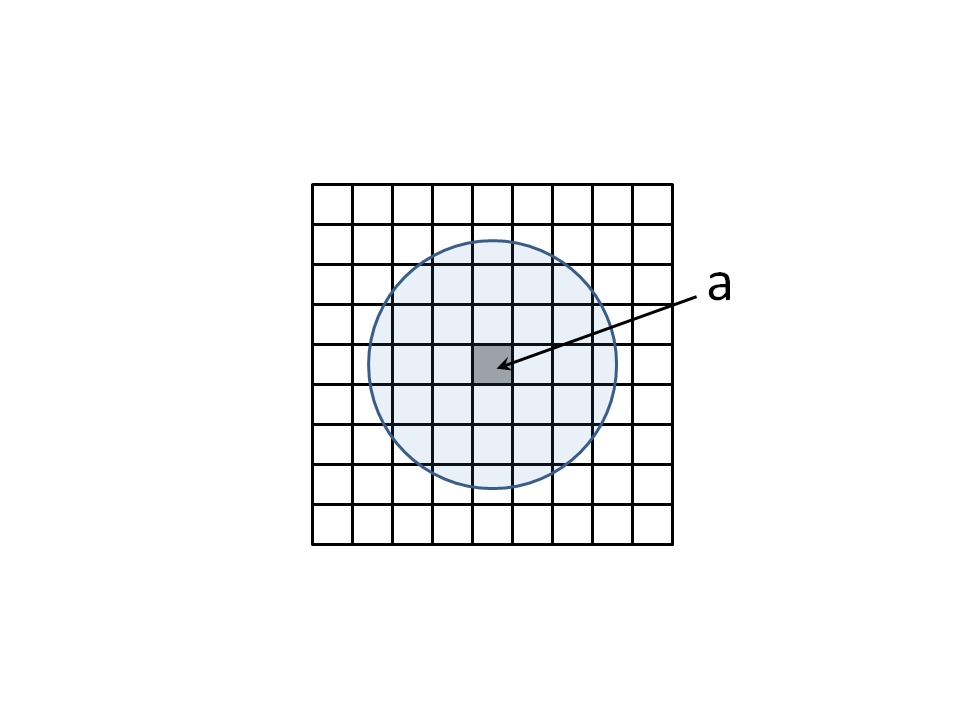
\includegraphics[width=170mm]{rs_kernel.png}
\caption{A visual depiction of the process used to select cells that were ``available" in spatio-temporal abundance models incorporating resource selection.  In particular, the redistribution kernels for the shaded cell $a$ only exhibited positive $\varphi_{a,b}$ values for cells $b$ that intersected with a 3-unit radius circle emanating from the centroid of $a$.} \label{fig:res-sel}
\end{center}
\end{figure*}

\begin{figure*}
\begin{center}
\includegraphics[width=170mm]{sim_generic_maps.pdf}
\caption{An example of one simulation iteration, whereby (a) a habitat covariate is simulated across a hypothetical landscape and allowed to evolve over time (top panels), (b) animal abundance is simulated conditional on the simulated habitat covariate and an assumed formulation for spatio-temporal dynamics, (c) transect surveys are simulated over the landscape (here, transects were assumed to cover $5\%$ of each grid cell transversed), and (d) animal abundance is estimated via a spatio-temporal statistical model.  Each column depicts results for a given time step (each simulation used 20 time steps).  In this particular simulation, abundance was simulated according to the closed population resource selection (CPRS) specification, while estimation was conducted assuming a closed population ideal free (CPIF) model.}
\label{fig:sim_maps}
\end{center}
\end{figure*}

\begin{figure*}
\begin{center}
\includegraphics[width=170mm]{bias_generic.pdf}
\caption{Boxplots depicting proportion relative bias of animal abundance for different combinations of data generating model (CPRD, CPUD, or OPRD), sampling effort (1 or 5 transects/time step), and estimation model for ``generic" simulations.  Proportion bias is computed by averaging bias of the posterior mean over all time steps for a particular simulation, with each simulation contributing one data point to each boxplot.  The lower and upper limits of each box correspond to first and third quartiles, while whiskers extend to the lowest and highest observed bias within 1.5 interquartile range units from the box.  Outliers outside of this range are denoted with points.  To make plots more legible, outliers with a proportional bias of greater than 2.0 were truncated at 2.0 for ``1 transect" simulations and at 0.25 for ``5 transect" simulations (denoted with open triangles). Horizontal lines within boxes denote median bias.  Note that the number of simulations for each boxplot varies by estimation model and number of transects (see XXX).
}
\label{fig:sim_maps}
\end{center}
\end{figure*}

\end{document}
